\documentclass[handout,compress]{beamer}

\usetheme[block=fill]{metropolis}

\usepackage{graphicx} % Allows including images
\usepackage{amsmath,amsfonts,amsthm,amssymb}
\usepackage{color}
\usepackage{xcolor,cancel}
\usepackage{multicol}

%\setitemize{label=\usebeamerfont*{itemize item}%
%	\usebeamercolor[fg]{itemize item}
%	\usebeamertemplate{itemize item}}
\definecolor{mDarkBrown}{HTML}{604c38}
\definecolor{mDarkTeal}{HTML}{23373b}
\definecolor{mLightBrown}{HTML}{EB811B}
\definecolor{mMediumBrown}{HTML}{C87A2F}
\definecolor{mygreen}{HTML}{98C2B9}
\definecolor{myyellow}{HTML}{DFD79C}
\definecolor{myblue}{HTML}{8CA7CC}
\definecolor{kern}{HTML}{8CC2B7}

\usepackage{float}
\usepackage{framed}
\usepackage{epsfig}
\usepackage{graphicx}
\usepackage{subcaption}
\usepackage{ulem}
\usepackage{hhline}
\usepackage{multirow}
\usepackage{comment}   
\usepackage{bbm}
\usepackage{tikz}   
\usepackage{ulem}
\def\Put(#1,#2)#3{\leavevmode\makebox(0,0){\put(#1,#2){#3}}}
\newcommand*\mystrut[1]{\vrule width0pt height0pt depth#1\relax}
\newcommand{\eqdef}{\mathbin{\stackrel{\rm def}{=}}}


\newcommand{\bs}[1]{\boldsymbol{#1}}
\newcommand{\bv}[1]{\mathbf{#1}}
\newcommand{\R}{\mathbb{R}}
\newcommand{\E}{\mathbb{E}}

\DeclareMathOperator*{\argmin}{arg\,min}
\DeclareMathOperator*{\argmax}{arg\,max}
\DeclareMathOperator{\nnz}{nnz}
\DeclareMathOperator{\Var}{Var}
\DeclareMathOperator{\sinc}{sinc}
\DeclareMathOperator{\mv}{mv}
\DeclareMathOperator{\sgn}{sgn}
\DeclareMathOperator{\step}{step}
\DeclareMathOperator{\gap}{gap}
\DeclareMathOperator{\poly}{poly}
\DeclareMathOperator{\tr}{tr}
\DeclareMathOperator{\orth}{orth}
\newcommand{\norm}[1]{\|#1\|}
\captionsetup[subfigure]{labelformat=empty}
\captionsetup[figure]{labelformat=empty}
\DeclareMathOperator*{\lmin}{\lambda_{min}}
\DeclareMathOperator*{\lmax}{\lambda_{max}}

\newcommand{\specialcell}[2][c]{%
	\begin{tabular}[#1]{@{}c@{}}#2\end{tabular}}
\newcommand{\specialcellleft}[2][c]{%
	\begin{tabular}[#1]{@{}l@{}}#2\end{tabular}
}

\usepackage{tabstackengine}
\stackMath

\newtheorem{claim}[theorem]{Claim}


%----------------------------------------------------------------------------------------
%	TITLE PAGE
%----------------------------------------------------------------------------------------

\title{CS-UY 4563: Lecture 24 \\ Reinforcement Learning}
\author{NYU Tandon School of Engineering, Prof. Christopher Musco}
\date{}

\begin{document}
	
	\begin{frame}
		\titlepage 
	\end{frame}
	
	\metroset{titleformat=smallcaps}
	


\begin{frame}
	\frametitle{some material we didn't have time for}
	\textbf{Supervised learning:}
	\begin{itemize}
		\item \textbf{Decision trees.} Very effective model for problems with few features. Difficult to train, but heuristics work well in practice.
		\item \textbf{Boosting.} Approach for combining several ``weak" models to obtain better overall accuracy than any one model alone.
	\end{itemize}
	\textbf{Unsupervised learning:}
	\begin{itemize}
	\item \textbf{Adversarial models.} Modern alternative to auto-encoders that performs very well for lots of interesting problems, especially in generative ML. 
	\item \textbf{\alert{Clustering.}} Hugely important for data exploration and visualization. 
\end{itemize}
\end{frame}
	
\begin{frame}
	\frametitle{data clustering}
	\textbf{Important unsupervised learning task:} 
	\begin{center}
		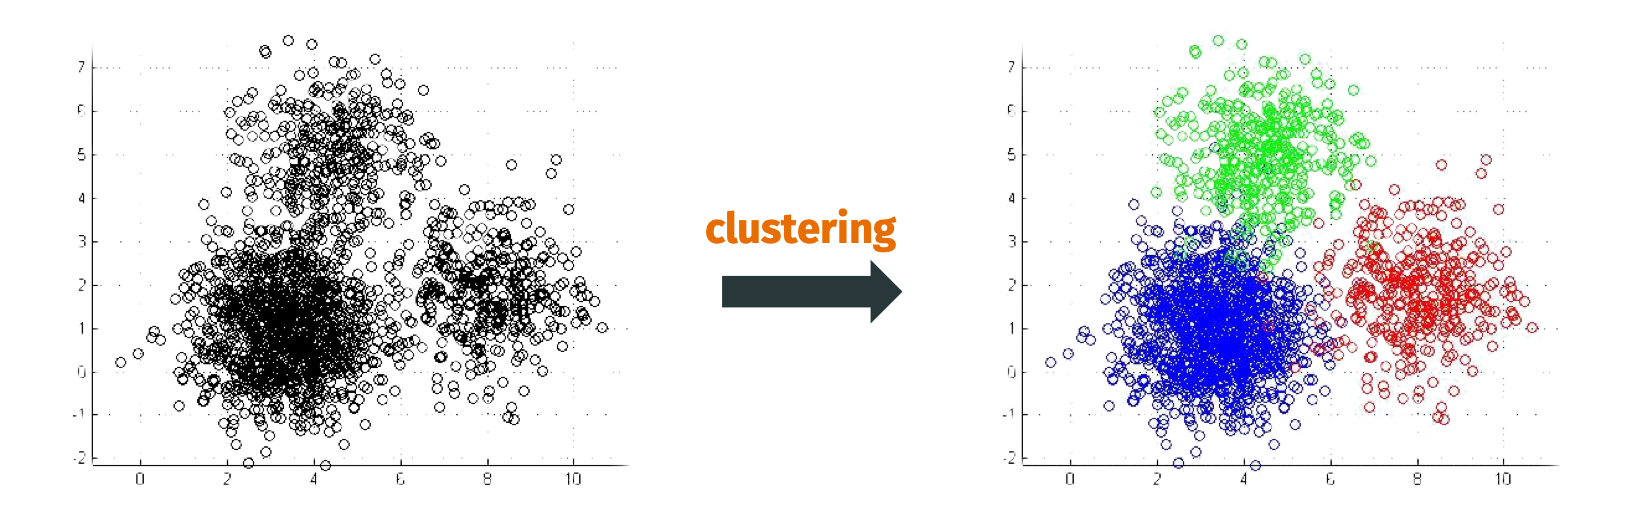
\includegraphics[width=\textwidth]{clustering_obj.png}
	\end{center}
Separate unlabeled data into natural clusters.
\begin{itemize}
	\item Exploratory data analysis. 
	\item Categorizing and grouping data. 
	\item Visualizing data. 
\end{itemize}
\end{frame}

\begin{frame}
	\frametitle{data clustering}
	\textbf{Example application:}
	\begin{center}
		\textbf{Images of Cats}.\vspace{-.5em}
		
		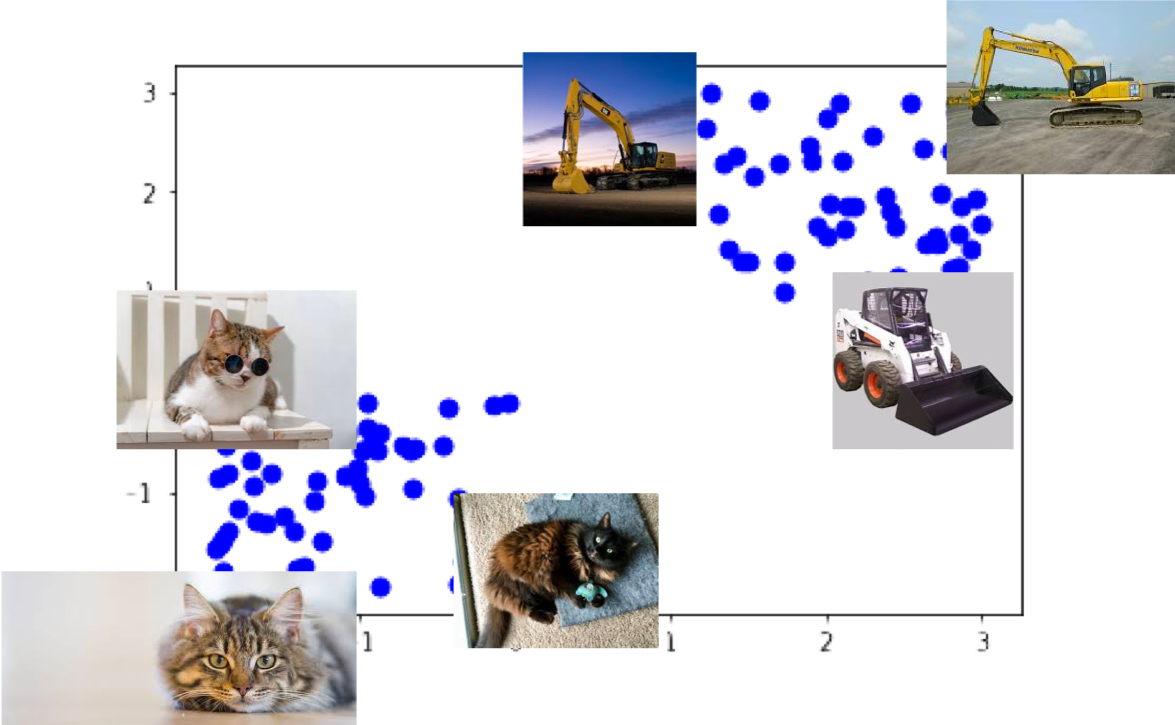
\includegraphics[width=.65\textwidth]{clustering_use.png}
	\end{center}
	Find sub-classes in your data which you did not know about. Helps you decide how to adjust features or improve data set for a supervised application.
\end{frame}

\begin{frame}
	\frametitle{data clustering}
	\begin{center}
		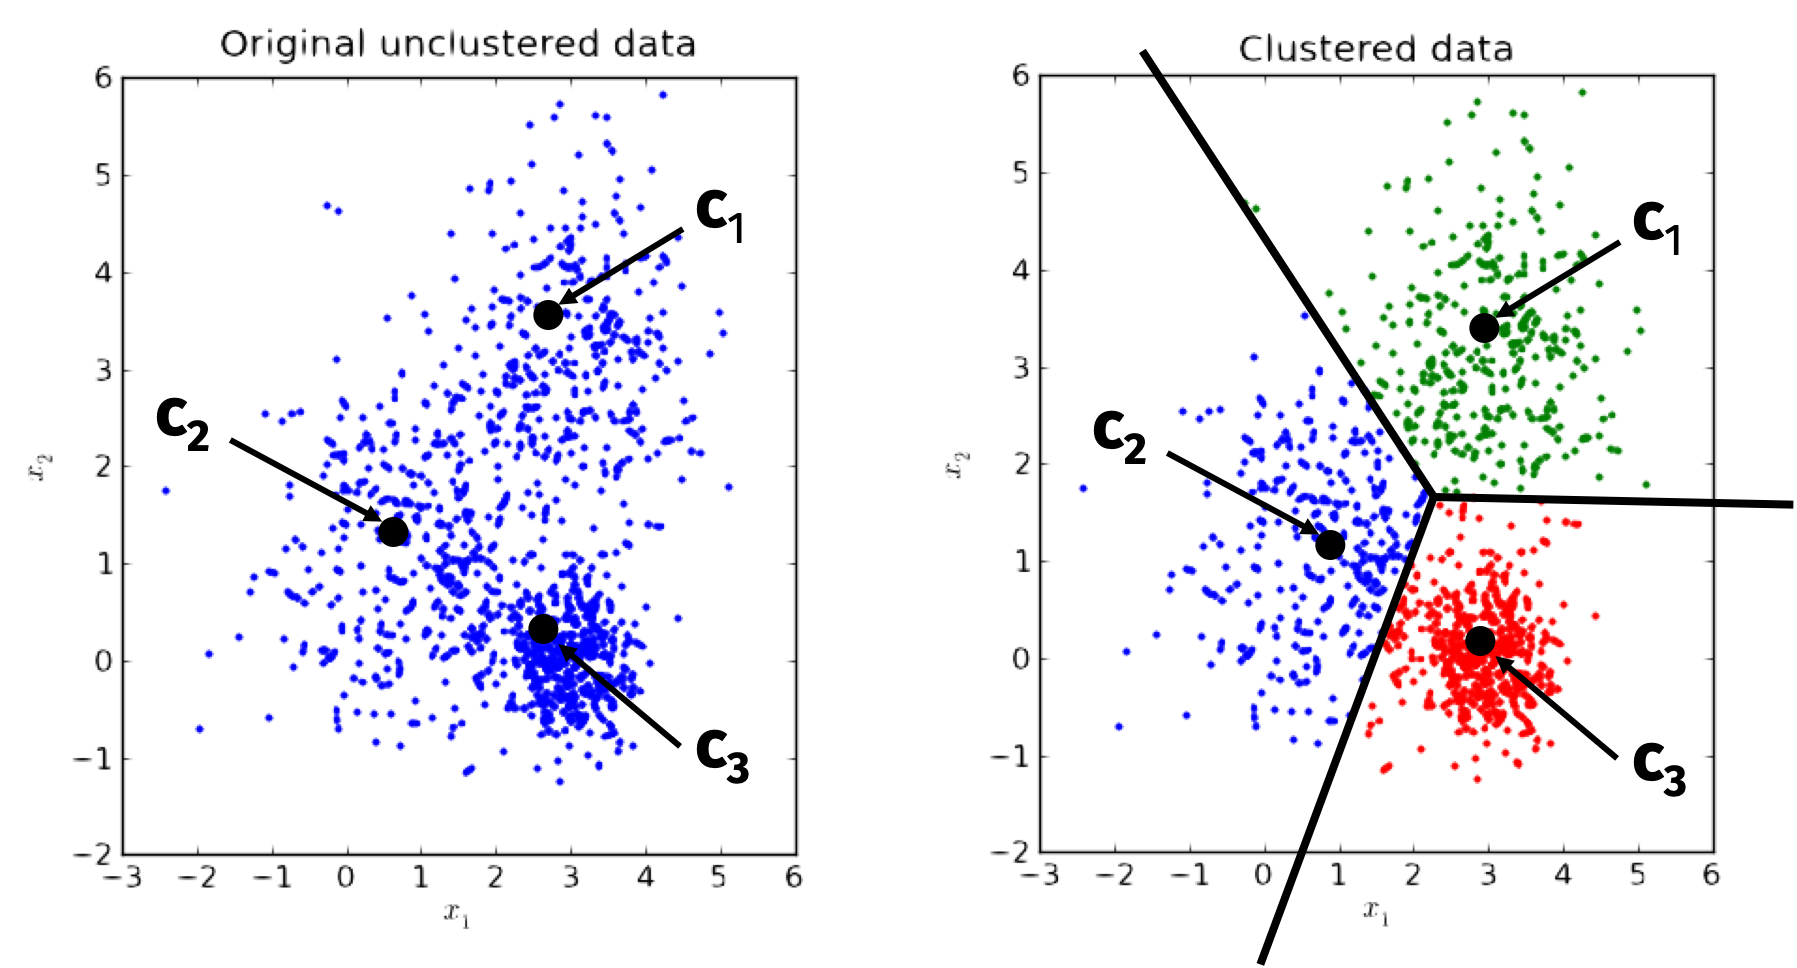
\includegraphics[width=.8\textwidth]{kcenter_clustering.png}
	\end{center}
	\textbf{k-center clustering:}
	\begin{itemize}
		\item Choose centers $\vec{c}_1, \ldots, \vec{c}_k \in \R^d$. 
		\item Assign data point $\vec{x}$ to cluster $i$ if 
		$\vec{c}_i$ is the ``nearest'' center. 
		\item Can use any distance metric.
	\end{itemize}
\end{frame}

\begin{frame}
	\frametitle{k-center clustering}
	Given data points $\vec{x}_1, \ldots, \vec{x}_n$ and distance metric $\Delta(\vec{x},\vec{c})\rightarrow \R$, choose $\vec{c}_1, \ldots, \vec{c}_k$ to minimize:
	\begin{align*}
	Cost(\vec{c}_1, \ldots, \vec{c}_k) = \sum_{i=1}^n \min_j \Delta(\vec{x}_i,\vec{c}_j).
	\end{align*}
	In general this could be a hard optimization problem.
\end{frame}

\begin{frame}
	\frametitle{k-means clustering}
	\small
	\textbf{Common choice:} Use Euclidean distance. I.e. set $\Delta(\vec{x},\vec{c}) = \|\vec{x} - \vec{c}\|_2^2$.
	
	\begin{itemize}
		\item If $k = 1$, optimal choice for $c_1$ is the centroid $\frac{1}{n}\sum_{i=1}^n \vec{x}_n$. For large $k$ the problem is NP-hard.
		\item Can be solved efficiently in practice using optimization techniques known as \textbf{alternating minimization}. Called ``Llyod's algorithm'' when applied to $k$-means clustering. 
		\item Euclidean $k$-means can only identify \emph{linearly separable clusters}.
	\end{itemize}
	\begin{center}
	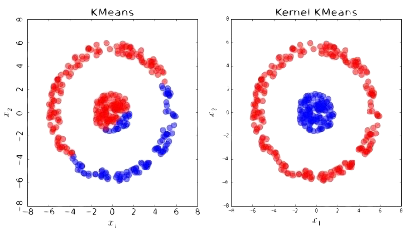
\includegraphics[width=.6\textwidth]{kmeans_vs_kernel.png}
\end{center}
\end{frame}

\begin{frame}
	\frametitle{reinforcement learning}
	\alert{\textbf{Today:} Give flavor of the area and insight into \emph{one} algorithm (Q-learning) which has been successful in recent years.}
	
	\textbf{Basic setup:\footnote{Slide content adapted from: \url{http://cs231n.stanford.edu/}}}
	\begin{itemize}
		\item \textbf{Agent} interacts with \textbf{environment} over time $1, \ldots, t$.
		\item Takes repeated sequence of \textbf{actions}, $a_1, \ldots, a_t$ which effect the environment.
		\item \textbf{State} of the environment over time denoted $s_1, \ldots, s_t$.
		\item Earn \textbf{rewards} $r_1, \ldots, r_t$ depending on actions taken and states reached.
		\item Goal is to maximize reward over time. 
	\end{itemize}
\end{frame}


\begin{frame}
	\frametitle{reinforcement learning examples}
	\small
	Classic inverted pendulum problem:
	\begin{center}
		\includegraphics*[width=.3\textwidth]{cart.png}
	\end{center}
\begin{multicols}{2}
	\begin{itemize}
		\item \textbf{Agent:} Cart/software controlling cart.
		\item \textbf{State:} Position of the car, pendulum head, etc. 
		\vspace{3em}
		
		\item \textbf{Actions:} Move cart left or move right.
		\item \textbf{Reward:} 1 for every time step that $|\theta| < 90^\circ$ (pendulum is upright). $0$ when $|\theta| = 90^\circ$
	\end{itemize}
\end{multicols}
\end{frame}

\begin{frame}
	\frametitle{reinforcement learning examples}
			\small
	This problem has a long history in \textbf{Control Theory.} Other applications of classical control:
	\begin{itemize}
		\item Semi-autonomous vehicles (airplanes, helicopters, rockets, etc.)
		\item Industrial processes (e.g. controlling large chemical reactions)
		\item Robotics
	\end{itemize}
	\begin{center}		
		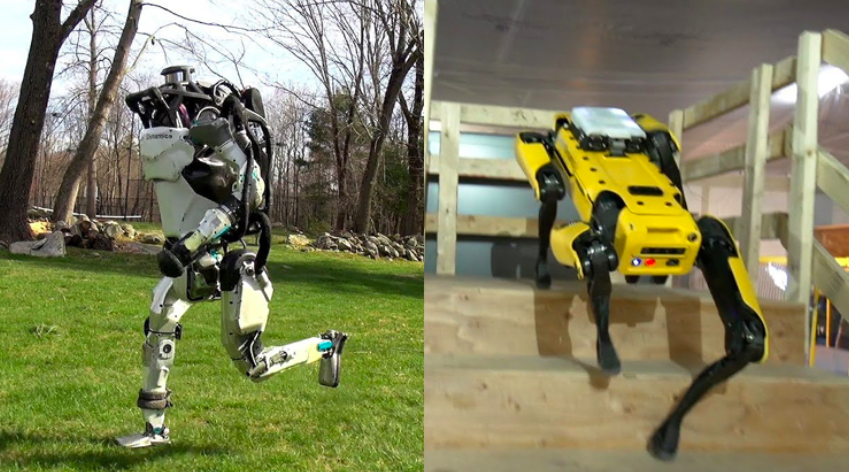
\includegraphics[width=.5\textwidth]{boston.png}
		
		control theory : reinforcement learning :: stats : machine learning
	\end{center}
\end{frame}


\begin{frame}
	\frametitle{reinforcement learning examples}
	\small
	Strategy games, like Go:
	\begin{center}
		\includegraphics*[width=.5\textwidth]{alpah_go.jpg}
	\end{center}
	\begin{multicols}{2}
		\begin{itemize}
			\item \textbf{State:} Position of all pieces on board.
			\item \textbf{Actions:} Place new piece.
			\item \textbf{Reward:} $1$ if in winning position at time $t$. $0$ otherwise.
		\end{itemize}
	\end{multicols}
This is a \emph{sparse reward problem}. Payoff only comes after many times steps, which makes the problem very challenging.
\end{frame}

\begin{frame}
	\frametitle{reinforcement learning examples}
	\small
	Video games, like classic Atari games:
	\begin{center}
		\includegraphics*[width=.8\textwidth]{atari_full.png}
	\end{center}
	\begin{multicols}{2}
		\begin{itemize}
			\item \textbf{State:} Raw pixels on the screen (sometimes there is also hidden state which can't be observed by the player). 
			\item \textbf{Actions:} Actuate controller (up,down,left,right,click).
			\item \textbf{Reward:} $1$ if point scored at time $t$. 
		\end{itemize}
	\end{multicols}
	
\end{frame}

\begin{frame}
	\frametitle{mathematical framework for rl}
	\small
	Model problem as a \textbf{Markov Decision Process (MDP)}:
	\begin{itemize}
		\item $\mathcal{S}:$ Set of all possible states. $|\mathcal{S}| = n$. 
		\item $\mathcal{A}:$ Set of all possible actions. $|\mathcal{A}| = k$. 
		\item \textbf{Reward function} $R(s,a): \mathcal{S}\times \mathcal{A} \rightarrow \text{ probability distribution over $\R$.}$ $r_t \sim R(s_t, a_t)$. 
		\item \textbf{State transition function} $P(s,a): \mathcal{S}\times \mathcal{A} \rightarrow \text{ probability distribution over $\mathcal{S}$.}$ $s_{t+1} \sim P(s_t, a_t)$. 
 	\end{itemize}
\begin{center}
	\alert{Why is this called a \emph{Markov} decision process? What does the term Markov refer to?}
\end{center}
\end{frame}

\begin{frame}
	\frametitle{mathematical framework for rl}
	\textbf{Goal:} Learn a \textbf{policy} $\Pi: \mathcal{S} \rightarrow \mathcal{A}$ from states to actions which maximized expected cumulative reward.
	\begin{itemize}
		\item Start is state $s_0$. 
		\item For $t = 0\ldots, T$
		\begin{itemize}
			\item $r_t \sim R(s_t,\Pi(s_t))$.
			\item $s_{t+1} \sim P(s_t,\Pi(s_t))$.
		\end{itemize}
	\end{itemize}	
The \textbf{time horizon} $T$ could be finite (game with fixed number of steps) or infinite (stock investing). Goal is to maximize:
\begin{align*}
reward(\Pi) = \E \sum_{t = 0}^T r_t
\end{align*}
$[s_0,a_0, r_0], [s_1, a_1, r_1], \ldots, [s_t, a_t, r_t]$ is called a \textbf{trajectory} of the MDP under policy $\Pi$. 
\end{frame}

\begin{frame}
	\frametitle{simple example: gridworld}
	\begin{center}
		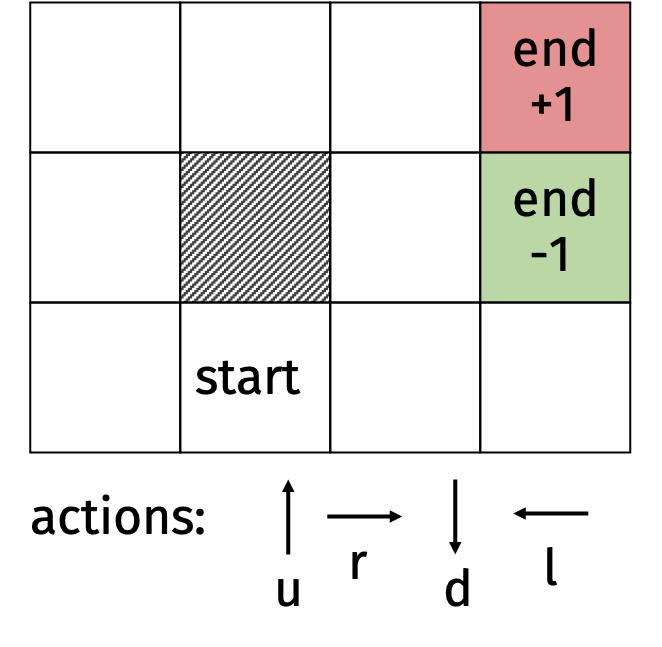
\includegraphics[width=.5\textwidth]{gridworld.png}

\vspace{-.5em}
	\begin{itemize}
		\item $r_t = -.01$ if not at an end position. $\pm 1$ if at end position.
		\item $P(s_t, a):$ $50\%$ of the time move in the direction indicated by $a$. $50\%$ of the time move in a random direction.   
	\end{itemize}
	\alert{\textbf{What is the optimal policy $\Pi$?}}
	\end{center}
\end{frame}


\begin{frame}
	\frametitle{simple example: gridworld}
	\begin{center}
		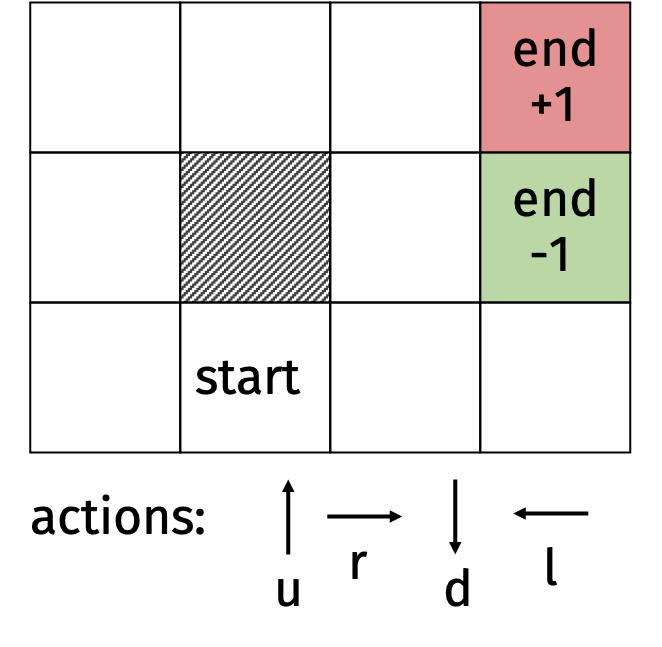
\includegraphics[width=.5\textwidth]{gridworld.png}
		
		\vspace{-.5em}
		\begin{itemize}
			\item $r_t = -.5$ if not at an end position. $\pm 1$ if at end position.
			\item $P(s_t, a):$ $50\%$ of the time move in the direction indicated by $a$. $50\%$ of the time move in a random direction.   
		\end{itemize}
		\alert{\textbf{What is the optimal policy $\Pi$?}}
	\end{center}
\end{frame}

\begin{frame}
	\frametitle{discount factor}
	For infinite or very long times horizon games (large $T$), we often introduce a \textbf{discount factor} $\gamma$ and seek instead to find a policy $\Pi$ which minimizes:
	\begin{align*}
	\E \sum_{t = 0}^T \gamma^t r_t
	\end{align*}
	where $r_t \sim R(s_t,\Pi(s_t))$ and $s_{t+1} \sim P(s_t,\Pi(s_t))$ as before. 
	
	From now on assume $T = \infty$. We can do this without loss of generality by adding a time parameter to state and moving into an ``end state'' with no additional rewards once the time hits $T$. 
\end{frame}

\begin{frame}
	\frametitle{value function and q function}
	Two important definitions. 
	\begin{itemize}
		\item \textbf{Value function:} $V^\Pi(s) = \E_{\Pi,s_0 = s} \sum_{t\geq 0}\gamma^t r_t$. Measures the expected return if we start in state $s$ and follow policy $\Pi$. 
		\item \textbf{$Q$-function: $Q^\Pi(s,a) = \E_{\Pi,s_0 = s, a_0 = a} \sum_{t\geq 0}\gamma^t r_t$.} Measures the expected return if we start in state $s$, play action $a$, and then follow policy $\Pi$. 
	\end{itemize}
\begin{align*}
	Q^*(s,a)= \max_\Pi \E_{\Pi,s_0 = s, a_0 = a} \sum_{t\geq 0}\gamma^t r_t.
\end{align*}
\alert{If we knew the function $Q^*$, we would immediately know an optimal policy. Whenever we're in state $s$, we should always play action $a^* = \argmax_ Q^*(s,a)$.}
\end{frame}

\begin{frame}
	\frametitle{bellman equation}
	$Q^*$ satisfies what's known as a Bellman equation:
	\begin{align*}
	Q^*(s,a) = \E_{s' \sim P(s,a)} \left[R(s,a) + \gamma \max_{a'}Q^*(s',a')\right].
	\end{align*}
	\textbf{Value Iteration:} Used \emph{fixed point} iteration to find $Q^*$:
	\begin{itemize}
		\item Initialize $Q^0$ (e.g. randomly).
		\item For $i=1,\ldots, z$:
		\begin{itemize}
			\item $Q^{i} = \E_{s' \sim P(s,a)} \left[R(s,a) + \gamma \max_{a'}Q^{i-1}(s',a')\right]$
		\end{itemize}
	\end{itemize}
Possible to prove that $Q^i \rightarrow Q^*$ as $i \rightarrow \infty$.
\begin{center}
	\alert{Note that \emph{many} details are involved in this computation.}
	
	Need to handle the expectations on the right hand side by randomly sampling trajectories from the MDP.
\end{center}
\end{frame}

\begin{frame}
	\frametitle{central issue in reinforcement learning}
	\textbf{Bigger issue:} Even writing down $Q^*$ is intractable... This is a function over \alert{$|\mathcal{S}|^{|\mathcal{A}|}$} possible inputs. Even for relatively simple games, $|\mathcal{S}|$ is gigantic...
	
	Back of the envelope calculations:
	\begin{itemize}
		\item \textbf{Tic-tac-toe:} $3^{(3\times 3)} \approx 20,000$
		\item \textbf{Chess:} $\approx 10^{43}$ (due to Claude Shannon).
		\item \textbf{Go:} $3^{(19*\times19)} \approx 10^{171}$.
		\item \textbf{Atari:} $128^{(210\times 160)} \approx 10^{71,000}$.
	\end{itemize}
Number of atoms in the universe: $\approx 10^{82}$.
\end{frame}

\begin{frame}
	\frametitle{machine learning approach}
	Learn a \textbf{simpler} function $Q(s,a,{\theta}) \approx Q^*(s,a)$ parameterized by a small number of parameters ${\theta}$.  
	
	\textbf{Example:} Suppose our state can be represented by a vector in $\R^d$ and our action $a$ by an integer in $1,\ldots, |\mathcal{A}|$. We could use a linear function where $\theta$ is a small matrix:
	\begin{center}
		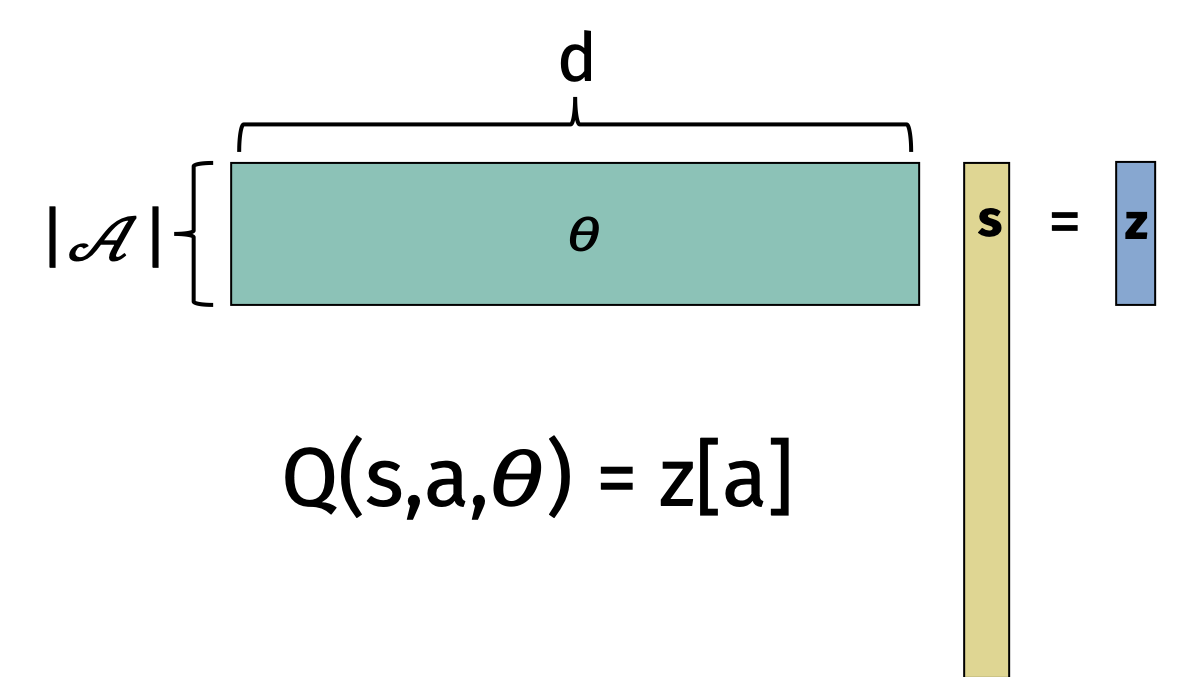
\includegraphics[width=.6\textwidth]{linear_example.png}
	\end{center}
\end{frame}

\begin{frame}
	\frametitle{machine learning approach}
	Learn a \textbf{simpler} function $Q(s,a,{\theta}) \approx Q^*(s,a)$ parameterized by a small number of parameters ${\theta}$.  
	
	\textbf{Example:} Could also use a (deep) neural network. 
	\begin{center}
		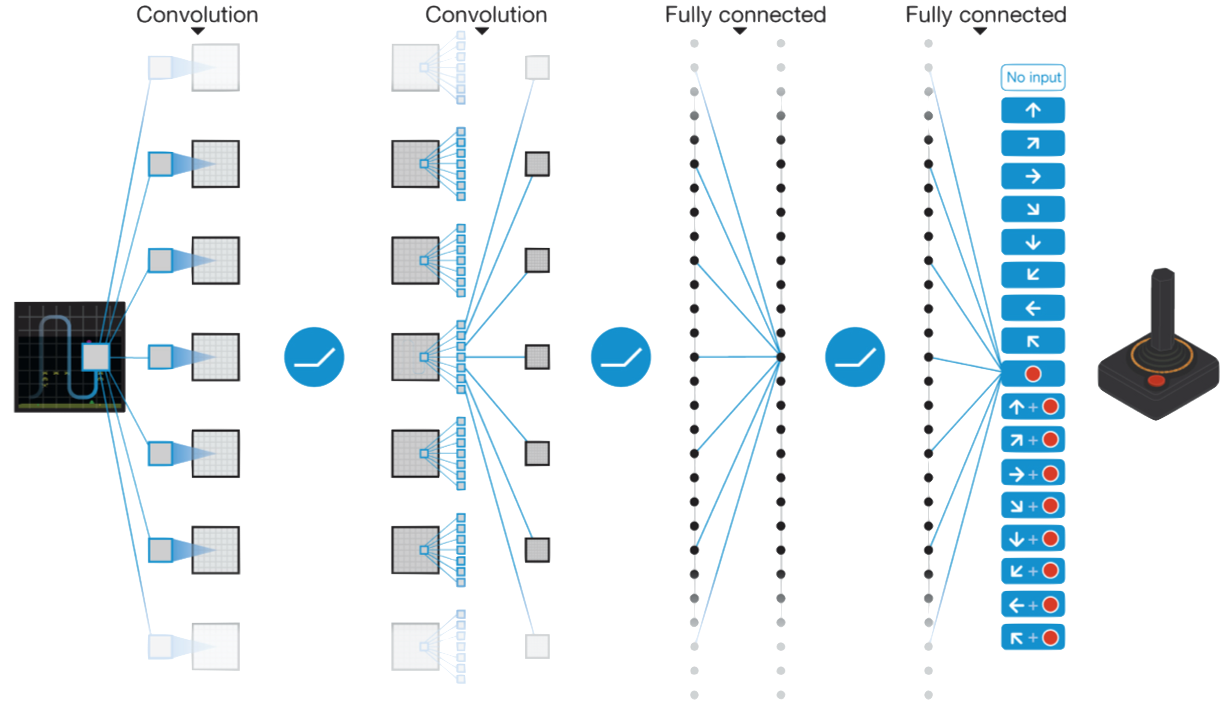
\includegraphics[width=.7\textwidth]{atari_func_approx.png}
	\end{center}
DeepMind: ``Human-level control through deep reinforcement learning'', Nature 2015.
\end{frame}

\begin{frame}
	\frametitle{machine learning approach}
	If $Q(s,a,\theta)$ is a good approximation to $Q^*(s,a)$ then we have an approximately optimal policy: $\tilde{\Pi}^*(s) = \argmax_a Q(s,a, \theta)$.
	\begin{itemize}
		\item Start in state $s_0$. 
		\item For $t = 1, 2, \ldots$
		\begin{itemize}
			\item $a^* = \argmax_a Q(s,a, \theta)$
			\item $s_{t} \sim P(s_{t-1},a^*)$
		\end{itemize}
	\end{itemize}
\begin{center}
	How do we find an optimal $\theta$? If we knew $Q^*(s,a)$ could use supervised learning, but the true $Q$ function is infeasible to compute. 
\end{center}
	
\end{frame}

\begin{frame}
	\frametitle{q-learning w/ function approximation}
	\textbf{Find $\theta$ which satisfies the Bellman equation:}
	\begin{align*}
	Q^*(s,a) &= \E_{s' \sim P(s,a)} \left[R(s,a) + \gamma \max_{a'}Q^*(s',a')\right]\\
	Q(s,a,\theta) &\approx \E_{s' \sim P(s,a)} \left[R(s,a) + \gamma \max_{a'}Q(s,a,\theta)\right].
	\end{align*} 
	
	Should be true for all $a,s$. Should also be true for $a,s \sim \mathcal{D}$ for any distribution $\mathcal{D}$:
	\begin{align*}
		\E_{s,a \sim \mathcal{D}} Q(s,a,\theta) &\approx \E_{s,a \sim \mathcal{D}}\E_{s' \sim P(s,a)} \left[R(s,a) + \gamma \max_{a'}Q(s,a,\theta)\right].
	\end{align*}
	\textbf{Loss function:}
	\begin{align*}
	L(\theta) = \E_{s,a \sim \mathcal{D}}\left(y - Q(s,a,\theta)\right)^2  
	\end{align*}
	where $y = 	\E_{s' \sim P(s,a)} \left[R(s,a) + \gamma \max_{a'}Q(s',a', \theta)\right]$. 
\end{frame}

\begin{frame}
	\frametitle{q-learning w/ function approximation}
	\small
	Minimize loss with \textbf{gradient descent}:
	\begin{align*}
	\nabla L(\theta) = -2\cdot \E_{s,a \sim \mathcal{D}} \nabla Q(s,a,\theta)\cdot \left[R(s,a) + \gamma \max_{a'}Q(s',a', \theta) - Q(s,a,\theta) \right]
	\end{align*}
	In practice use stochastic gradient:
	\begin{align*}
	\nabla L(\theta,s,a) = -2\cdot \nabla Q(s,a,\theta) \cdot \left[R(s,a) + \gamma \max_{a'}Q(s',a', \theta) - Q(s,a,\theta)\right]
	\end{align*}
	\begin{itemize}
		\item Initialize $\theta_0$
		\item For $i=0,1,2,\ldots $
		\begin{itemize}
			\item {Choose random $s,a \sim \mathcal{D}$.}
			\item Set $\theta_{i+1} = \theta_i - \eta\cdot\nabla L(\theta_i,s,a)$
		\end{itemize}
	\end{itemize}
where $\eta$ is a learning rate parameter.
\end{frame}
\begin{frame}
	\frametitle{q-learning w/ function approximation}
	\small
	\begin{itemize}
		\item Initialize $\theta_0$
		\item For $i=0,1,2,\ldots $
		\begin{itemize}
			\item \alert{Choose random $s,a \sim \mathcal{D}$.}
			\item Set $\theta_{i+1} = \theta_i - \nabla L(\theta_i,s,a)$.
		\end{itemize}
	\end{itemize}
What is the distribution $\mathcal{D}$?

\begin{itemize}
	\item \textbf{Random play}: Choose uniformly over reachable states + actions.
\end{itemize}
\textbf{Wasteful:} Seeks to approximate $Q^*$ well in parts of the state-action space that don't actually matter for optimal play. Would require a ton of samples. 
\end{frame}

\begin{frame}
	\frametitle{q-learning w/ function approximation}
	\textbf{More common approach:}
	Play according to current guess for optimal policy, with some random ``off-policy'' exploration. The $\mathcal{D}$ is the distribution over states/actions results form this play. Note that  $\mathcal{D}$ changes over time... 
	
	\textbf{$\epsilon$-greedy approach:}
	\begin{itemize}
		\item Initialize $s_0$.
		\item For $t=0, 1,2, \ldots, $
		\begin{itemize}
			\item $a_i = \begin{cases}\argmax_a Q(s_t,a, \theta_{curr}) & \text{with probabilty $(1-\epsilon)$}\\ \text{random action} & \text{with probabilty $\epsilon$} \end{cases}$ 
		\end{itemize}
	\end{itemize}
Exploration-exploitation tradeoff. Increasing $\epsilon$ = more \textbf{exploration}. 
\end{frame}

\begin{frame}
	\frametitle{references}
	\small
	Lots of other details we don't have time for! References:
	\begin{itemize}
		\item Original DeepMind Atari paper: \url{https://www.cs.toronto.edu/~vmnih/docs/dqn.pdf}, which is very readable.
		\item Stanford lecture video: \url{https://www.youtube.com/watch?v=lvoHnicueoE} and slides: \url{http://cs231n.stanford.edu/slides/2017/cs231n_2017_lecture14.pdf}
	\end{itemize}
	Important concept we did not cover: \textbf{experience replay}.
\end{frame}


\begin{frame}
	\frametitle{atari demo}
	\begin{center}
		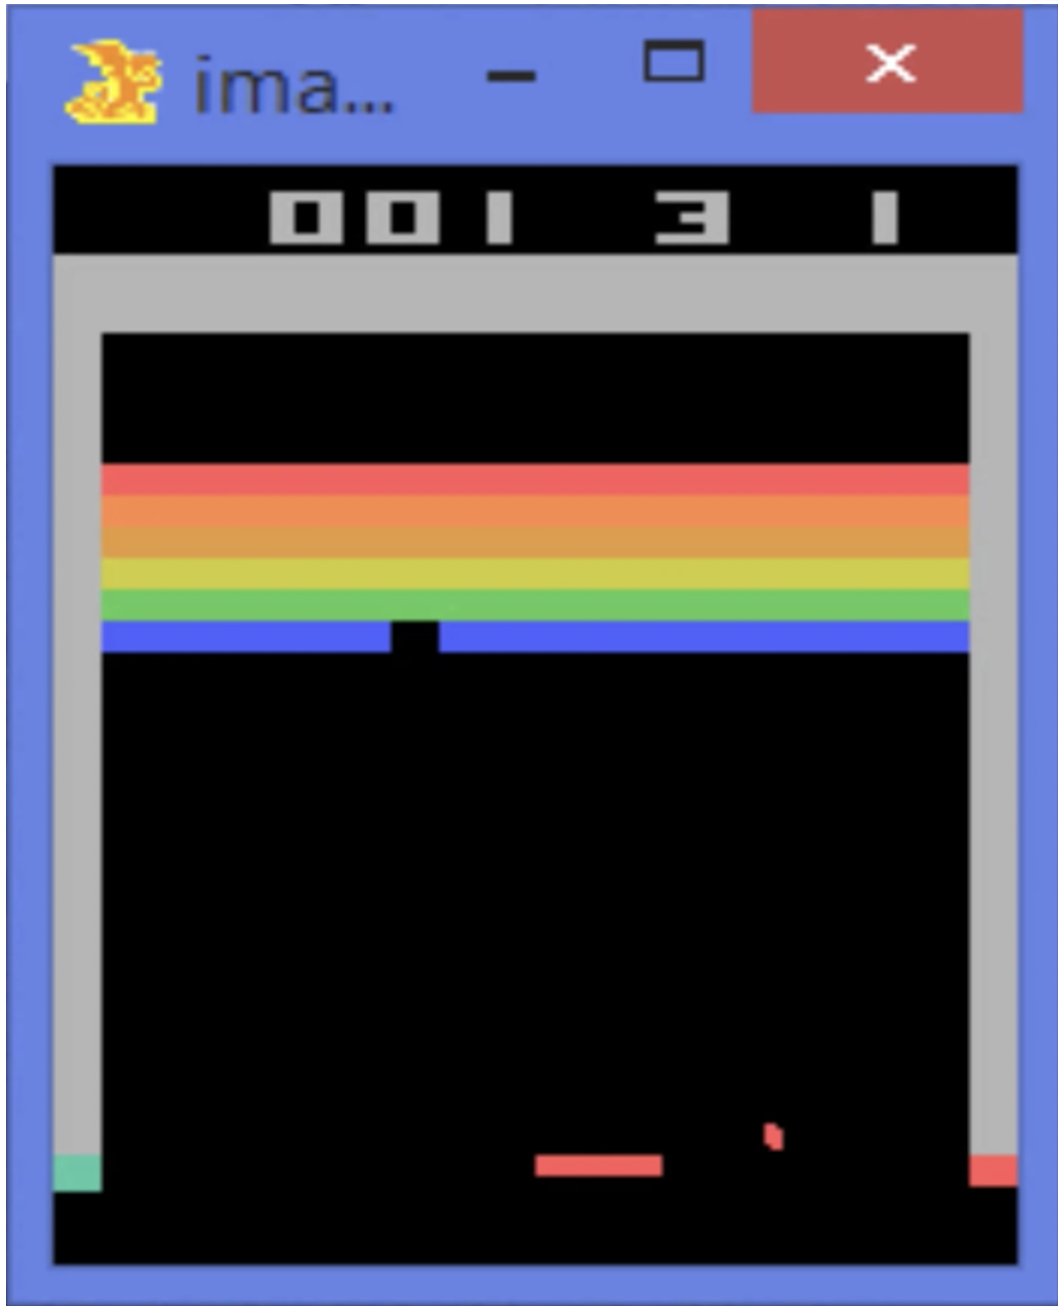
\includegraphics[width=.4\textwidth]{atari_game.png}
	\end{center}
	\url{https://www.youtube.com/watch?v=V1eYniJ0Rnk}
\end{frame}

\end{document} 



